\documentclass{article}
\usepackage[utf8]{inputenc}
\usepackage{polski}
\usepackage{geometry}
\usepackage{pdfpages}
\usepackage{pdfpages}
\usepackage{listings}
\usepackage{listingsutf8}
\usepackage{multirow}
\usepackage{siunitx}
\usepackage{multirow}
\usepackage{booktabs}
\usepackage{tabularx}
\usepackage{placeins}
\usepackage{pdflscape}
\usepackage{graphicx}
\usepackage{subfig}
\usepackage{hyperref}
\usepackage{amsmath}
\usepackage{colortbl}
\usepackage{listings}

\geometry{
a4paper,
total={170mm,257mm},
left=20mm,
top=20mm
}

\newcolumntype{Y}{>{\centering\arraybackslash}X}
\renewcommand\thesection{}
\renewcommand\thesubsection{}

\lstset{%
literate=%
 {ą}{{\k{a}}}1
 {ę}{{\k{e}}}1
 {Ą}{{\k{A}}}1
 {Ę}{{\k{E}}}1
 {ś}{{\'{s}}}1
 {Ś}{{\'{S}}}1
 {ź}{{\'{z}}}1
 {Ź}{{\'{Z}}}1
 {ń}{{\'{n}}}1
 {Ń}{{\'{N}}}1
 {ć}{{\'{c}}}1
 {Ć}{{\'{C}}}1
 {ó}{{\'{o}}}1
 {Ó}{{\'{O}}}1
 {ż}{{\.{z}}}1
 {Ż}{{\.{Z}}}1
 {ł}{{\l{}}}1
 {Ł}{{\l{}}}1
}
\lstset{ 
    backgroundcolor=\color{white},   % choose the background color; you must add \usepackage{color} or \usepackage{xcolor}; should come as last argument
    basicstyle=\footnotesize,        % the size of the fonts that are used for the code
    breakatwhitespace=false,         % sets if automatic breaks should only happen at whitespace
    breaklines=true,                 % sets automatic line breaking
    captionpos=b,                    % sets the caption-position to bottom
    commentstyle=\color{mygreen},    % comment style
    deletekeywords={...},            % if you want to delete keywords from the given language
    escapeinside={\%*}{*)},          % if you want to add LaTeX within your code
    %extendedchars=true,              % lets you use non-ASCII characters; for 8-bits encodings only, does not work with UTF-8
    firstnumber=1000,                % start line enumeration with line 1000
    frame=single,	                   % adds a frame around the code
    keepspaces=true,                 % keeps spaces in text, useful for keeping indentation of code (possibly needs columns=flexible)
    keywordstyle=\color{blue},       % keyword style
    language=Octave,                 % the language of the code
    morekeywords={*,...},            % if you want to add more keywords to the set
    numbers=left,                    % where to put the line-numbers; possible values are (none, left, right)
    numbersep=5pt,                   % how far the line-numbers are from the code
    numberstyle=\tiny\color{mygray}, % the style that is used for the line-numbers
    rulecolor=\color{black},         % if not set, the frame-color may be changed on line-breaks within not-black text (e.g. comments (green here))
    showspaces=false,                % show spaces everywhere adding particular underscores; it overrides 'showstringspaces'
    showstringspaces=false,          % underline spaces within strings only
    showtabs=false,                  % show tabs within strings adding particular underscores
    stepnumber=2,                    % the step between two line-numbers. If it's 1, each line will be numbered
    stringstyle=\color{mymauve},     % string literal style
    tabsize=2,	                   % sets default tabsize to 2 spaces
    title=\lstname                   % show the filename of files included with \lstinputlisting; also try caption instead of title
}
\lstset{language=python}

\title{Teoria współbieżności\\ 
Laboratorium XII}
\author{Maciej Trątnowiecki}
\date{AGH, Semestr Zimowy, 2020/2021}

\begin{document}
    \maketitle
    \section{Implementacja}
        \subsection{Relacja zależności D}
            \begin{lstlisting}
    @staticmethod
    def __not_in(key, value, rel):
        return (key not in rel) or (value not in rel[key])

    @staticmethod
    def __safe_add(key, val, rel):
        if key not in rel:
            rel[key] = set([val])
        else:
            rel[key].add(val)

    @property
    def dependency_relation(self):
        if self.__dependency_relation:
            return self.__dependency_relation

        def all_pairs(arr):
            for a in arr:
                for b in arr:
                    yield (a,b)

        dependency = {}
        for (a,b) in all_pairs(self.problem.alphabet):
            if self.__not_in(a,b,self.problem.relation):
                self.__safe_add(a,b,dependency)

        self.__dependency_relation = dependency
        return dependency
            \end{lstlisting}
        Dla wszystkich par znaków z alfabetu wejściowego wyznaczamy w relacji D te, które nie należą do relacji I. 
        
        \subsection{Ślad [w] względem relacji I}
            \begin{lstlisting}
    def get_trace(self, word=None, traces=None):
        word = word if word else self.problem.word
        traces = traces if traces else set()
        traces.add(word)
        i = 0
        while i < len(word) - 1:
            char = word[i]
            changed = word[:i] + word[i+1] + word[i] + word[i+2:]
            if not self.__not_in(char, word[i+1], self.problem.relation) \
                and changed not in traces:
                traces |= self.get_trace(word=changed, traces=traces)
                i+=1
            i+=1
        return traces
            \end{lstlisting}
            Algorytm rekurencyjny zamieniający pary znaków w słowie wejściowym. 
            
        \subsection{Postać normalna Foaty FNF([w]) śladu [w]}
            \begin{lstlisting}
    def get_foata(self):
        result = []
        stacks = {char: [] for char in self.problem.alphabet}

        for i in range(len(self.problem.word)-1, -1, -1):
            char = self.problem.word[i]
            stacks[char].append(char)
            for char2 in self.problem.alphabet:
                if char != char2 \
                    and self.__not_in(char, char2, self.problem.relation):
                    stacks[char2].append('#')

        while True:
            block = '('
            not_empty_stack = False
            popped_markers = {char: 0 for char in self.problem.alphabet}
            for key in stacks.keys():
                if len(stacks[key]) == 0:
                    continue
                not_empty_stack = True
                if stacks[key][-1] == '#' or popped_markers[key] != 0:
                    continue
                popped = stacks[key].pop()
                block+=popped
                for char in self.dependency_relation[popped]:
                    if char != popped \
                        and len(stacks[char]) != 0:
                        stacks[char].pop()
                        popped_markers[char]+=1

            block+=')'
            if not not_empty_stack:
                break
            result.append(block)

        return result
            \end{lstlisting}
            Algorytm pochodzący z \textit{Handbook of Formal Languages}. 
            
        \subsection{Graf zależności w postaci minimalnej dla słowa w}
            \begin{lstlisting}
class DependencyGraph(nx.DiGraph):
    def __init__(self, problem: Problem, dependency_relation, *args, **kwargs):
        super().__init__(directed=True, *args, **kwargs)
        self.problem = problem
        for i in range(len(problem.word)):
            self.add_node(i, char=problem.word[i])
            for j in range(i):
                t1 = self.node_char(j)
                t2 = self.node_char(i)
                if t1 in dependency_relation and t2 in dependency_relation[t1]:
                    self.add_edge(j,i)
        self.minimize()

    def minimize(self):
        for node in self.nodes:
            if not self.out_edges(node):
                continue
            delete = set()
            for neighbour in map(lambda x: x[1],self.out_edges(node)):
                if neighbour in delete:
                    continue
                visited = set()
                self.dfs(neighbour, visited)
                visited.remove(neighbour)
                delete |= set(visited_node for visited_node in visited)
            delete = filter(lambda e: self.contains_edge(e), map(lambda n: (node, n), delete))
            self.remove_edges_from(delete)

    def dfs(self, node, visited, topological=None):
        if node in visited:
            return
        visited.add(node)
        for out_edge in self.out_edges(node):
            neighbour = out_edge[1]
            if neighbour not in visited:
                self.dfs(neighbour, visited, topological=topological)
        if topological is not None:
            topological.append(node)

    def contains_edge(self, edge):
        return edge in self.edges

    def node_char(self, node):
        return nx.get_node_attributes(self, 'char')[node]
            \end{lstlisting}
            Początkowo algorytm w sposób naiwny tworzy prosty graf. Następnie minimalizuje go z wykorzystaniem algorytmu dfs, usuwając krawędzie pomiędzy wierzchołkiem a wierchołkami osiągalnymi z jego sąsiadów. 
            
        \subsection{Postać normalną Foaty na podstawie grafu}
            \begin{lstlisting}
    def get_foata(self):
        result = []
        topo = self.topological_sort()
        i = 0
        while i < len(self.problem.word):
            block = '('
            block += topo[i]

            k = i
            i += 1
            while i < len(self.problem.word):
                is_independent = True
                for j in range(k,i):
                    if (topo[i] not in self.problem.relation) \
                        or (topo[j] not in self.problem.relation[topo[i]]):
                        is_independent = False
                        break
                if is_independent:
                    block += topo[i]
                    i+=1
                else:
                    break
            block += ')'
            result.append(block)
        return result

    def topological_sort(self):
        visited = set()
        topo = []
        for node in self.nodes:
            self.dfs(node, visited, topological=topo)
        topo = list(map(lambda x: self.node_char(x), reversed(topo)))
        return topo
            \end{lstlisting}
            Graf zależności sortujemy topologicznie, następnie w kolejnośći topologicznej tworzymy postać Foaty. 
    
    \newpage
    \section{Wynik działania dla danych przykładowych}
        \subsection{Przykład 1}
            Dane testowe:
            $$
            A = {a, b, c, d}\quad
            I = {(a, d), (d, a), (b, c), (c, b)}\quad
            w = baadcb
            $$
            Wynik działania programu:
            \begin{lstlisting}
Dependency graph 
{'b': {'a', 'd', 'b'}, 
'd': {'d', 'c', 'b'}, 
'c': {'a', 'c', 'd'}, 
'a': {'a', 'c', 'b'}}
Traces {'bdaabc', 'badabc', 'bdaacb', 'baadbc', 'badacb', 'baadcb'}
Foata (b)(da)(a)(bc)
Foata (b)(da)(a)(bc)
            \end{lstlisting}
            \begin{figure}[h!]
                \centering
                \subfloat[Graf zależności]{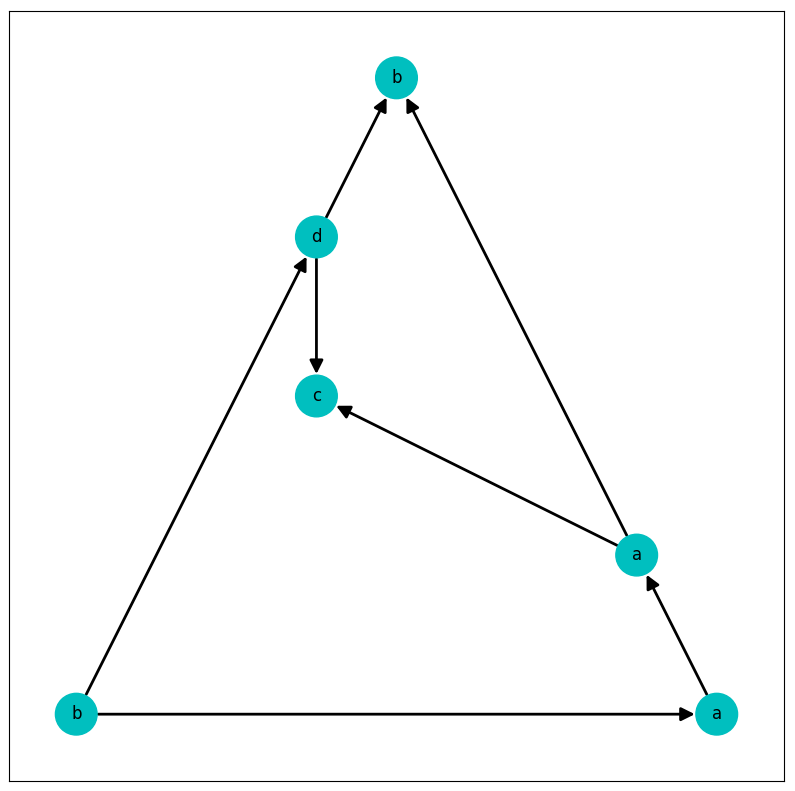
\includegraphics[width=10cm]{lab10/img/t0.png}}
                \caption{Przykład 1}
            \end{figure}
            
    \newpage
    \subsection{Przykład 2}
        Dane testowe:
        $$
        A = {a, b, c, d, e, f}\quad
        I = {(a, d), (d, a), (b, e), (e, b), (c, d), (d, c), (c, f), (f, c)}\quad
        w = acdcfbbe
        $$
        Wynik działania programu:
        \begin{lstlisting}
Dependency graph 
{'c': {'c', 'a', 'b', 'e'}, 
'b': {'c', 'b', 'a', 'd', 'f'}, 
'a': {'c', 'b', 'a', 'f', 'e'}, 
'd': {'d', 'b', 'e', 'f'}, 
'f': {'b', 'a', 'd', 'f', 'e'}, 
'e': {'c', 'a', 'd', 'f', 'e'}}        
Traces {'accdfebb', 'dafccbbe', 'dafccebb', 'acdfcbeb', 'acdfcbbe', 'daccfebb', 'accdfbeb', 'daccfbbe', 'dafccbeb', 'acdcfbbe', 'dacfcbbe', 'adfccebb', 'daccfbeb', 'dacfcbeb', 'adcfcebb', 'adccfbbe', 'adcfcbeb', 'adfccbbe', 'acdcfbeb', 'adccfebb', 'adccfbeb', 'acdfcebb', 'adcfcbbe', 'dacfcebb', 'adfccbeb', 'acdcfebb'}
Foata (ad)(cf)(c)(be)(b)
Foata (da)(fc)(c)(eb)(b)
        \end{lstlisting}
        \begin{figure}[h!]
            \centering
            \subfloat[Graf zależności]{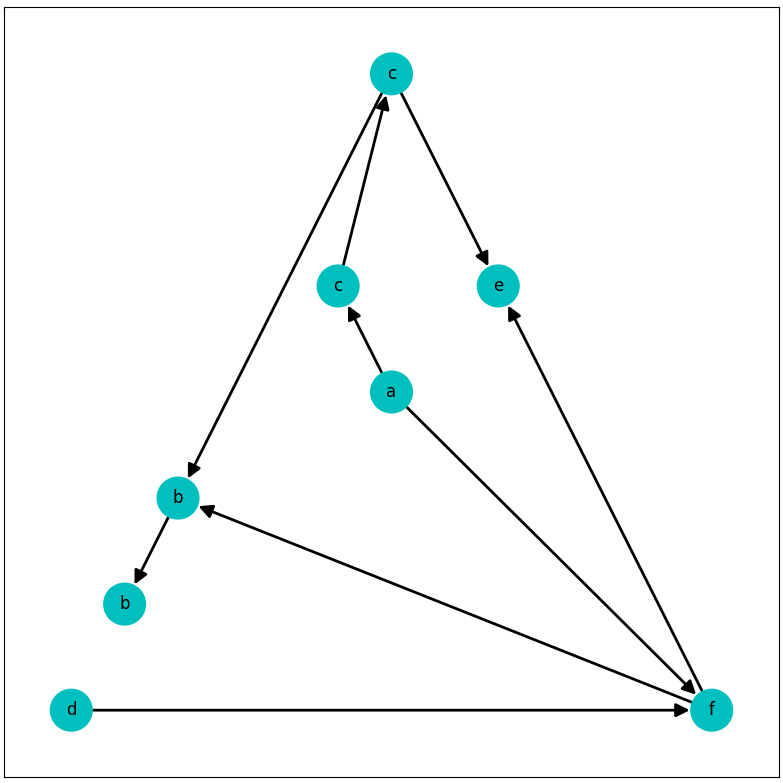
\includegraphics[width=10cm]{lab10/img/t1.png}}
            \caption{Przykład 2}
        \end{figure}

    \newpage
    \subsection{Przykład 3}
        Dane testowe:
        $$
        A = {a, b, c, d, e}\quad
        I = {(a, c), (c, a), (a, d), (d, a), (b, d), (d, b), (b, e), (e, b)}\quad
        w = acebdac
        $$
        Wynik działania programu:
        \begin{lstlisting}
Dependency graph 
{'e': {'e', 'a', 'c', 'd'}, 
'b': {'b', 'a', 'c'}, 
'a': {'e', 'b', 'a'}, 
'c': {'e', 'b', 'c', 'd'}, 
'd': {'e', 'c', 'd'}}
Traces {'caebdac', 'caedbac', 'cabeadc', 'acbedca', 'caebadc', 'cabedca', 'caebdca', 'acbedac', 'acbeadc', 'cabedac', 'acebadc', 'acebdac', 'acedbca', 'acebdca', 'acedbac', 'caedbca'}
Foata (ac)(eb)(ad)(c)
Foata (ca)(be)(ad)(c)
        \end{lstlisting}
        \begin{figure}[h!]
            \centering
            \subfloat[Graf zależności]{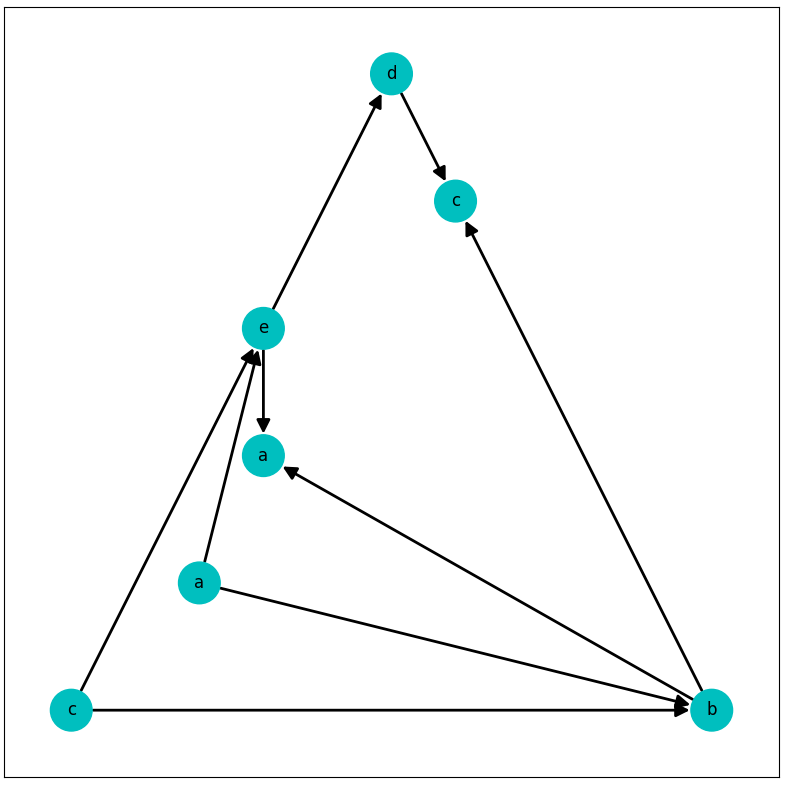
\includegraphics[width=10cm]{lab10/img/t2.png}}
            \caption{Przykład 3}
        \end{figure}

\end{document}